\documentclass[a3,convert]{standalone}
\usepackage{pgfplots}
\usepgfplotslibrary{smithchart}    
\usepgfplotslibrary{polar}   
\usepackage{siunitx} 
\usepackage{tikz}
\pgfplotsset{compat=1.18}
\usetikzlibrary{calc,intersections,through}
\usepackage{comment}

\begin{document}
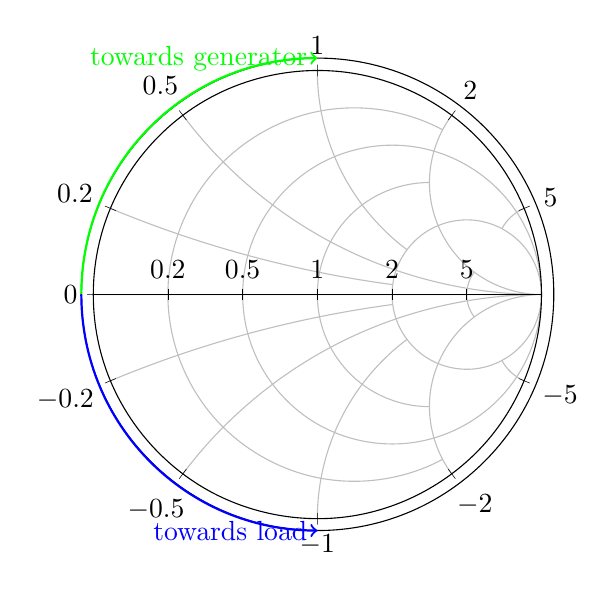
\begin{tikzpicture}
    \begin{smithchart}

        %\addplot[domain=0:10,samples=600,color=blue]{0.05};
        %\draw[dotted,blue,line width=2pt] (1,0) -- (200,0);
        %\draw[mark=*,only marks,mark options={solid},color={green},mark size=.2] (1,0) -- (0,0);
        %\addplot+[mark=*,only marks,samples at={0,.02,...,1},
        %    mark options={solid},color={green},mark size=.1,line width=1](x,0);
        %\addplot+[mark=*,only marks,samples at={5,-.1,...,1},
        %    mark options={solid},color={blue},mark size=.1,line width=1](x,0);

        %\addplot+[mark=*,only marks,samples at={0,.02,...,200},
        %    mark options={solid},color={red},mark size=.1,line width=1](0,x);
        %\addplot+[mark=*,only marks,samples at={0,-.02,...,-200},
        %    mark options={solid},color={red},mark size=.1,line width=1](0,x);

    \end{smithchart}
    
    % add rotation information
    \draw (2.85cm,2.85cm) circle (3cm);
    \draw[green,->,thick] (-0.15cm,2.85cm) .. controls (-0.15cm,4.515cm) and (1.185cm,5.85cm) .. (2.85cm,5.85cm)node[anchor=east]{towards generator};
    \draw[blue,->,thick] (-0.15cm,2.85cm) .. controls (-0.15cm,1.185cm) and (1.185cm,-0.15cm) .. (2.85cm,-0.15cm)node[anchor=east]{towards load};
\end{tikzpicture}
\end{document}